% Created 2020-02-23 Sun 11:08
% Intended LaTeX compiler: pdflatex

\documentclass[a4paper,12pt]{article}
\usepackage[margin=2cm]{geometry}

\usepackage{hyperref}
\usepackage[utf8]{inputenc}
\usepackage{fixltx2e}
\usepackage{graphicx}
\usepackage{longtable}
\usepackage{float}
\usepackage{wrapfig}
\usepackage{rotating}
\usepackage[normalem]{ulem}
\usepackage{amsmath}
\usepackage{textcomp}
\usepackage{marvosym}
\usepackage{wasysym}
\usepackage{multicol}
\usepackage{amssymb}
\tolerance=1000
\usepackage{listings}
\usepackage{xeCJK}
\setCJKmainfont{SimSun}
\usepackage{color}
\usepackage{listings}
\RequirePackage{fancyvrb}
\DefineVerbatimEnvironment{verbatim}{Verbatim}{fontsize=\small}
\lstset{basicstyle=\scriptsize\ttfamily}
\lstset{basicstyle=\tiny\ttfamily}
\usepackage{placeins}
\vspace{-0.2cm}
\usepackage{xcolor}
\definecolor{dkgreen}{rgb}{0,0.6,0}
\definecolor{dred}{rgb}{0.545,0,0}
\definecolor{dblue}{rgb}{0,0,0.545}
\definecolor{lgrey}{rgb}{0.9,0.9,0.9}
\definecolor{gray}{rgb}{0.4,0.4,0.4}
\definecolor{darkblue}{rgb}{0.0,0.0,0.6}
\definecolor{bubbles}{rgb}{0.91, 1.0, 1.0}
\lstdefinelanguage{python}{
backgroundcolor=\color{bubbles},
basicstyle=\footnotesize \ttfamily \color{black} \bfseries,
breakatwhitespace=false,
breaklines=true,
captionpos=b,
commentstyle=\color{dred},
deletekeywords={...},
escapeinside={\%*}{*)},
frame=single,
language=C++,
keywordstyle=\color{purple},
morekeywords={BRIEFDescriptorConfig,string,TiXmlNode,DetectorDescriptorConfigContainer,istringstream,cerr,exit},
identifierstyle=\color{black},
stringstyle=\color{blue},
rulecolor=\color{black},
showspaces=false,
showstringspaces=false,
showtabs=false,
stepnumber=1,
tabsize=5,
title=\lstname,
}
\usepackage{enumitem}
\setenumerate{noitemsep}
\setenumerate{nolistsep}
\setitemize{nolistsep}
\usepackage[compact]{titlesec}
\usepackage[utf8]{inputenc}
\vspace{-\topsep}
\author{yen yung chin}
\date{\today}
\title{Python programming}
\begin{document}

\maketitle
\tableofcontents


\section{變數、資料型態、輸出輸入}
\label{sec:org0fd8818}
\subsection{變數}
\label{sec:org4ab85f2}
\subsubsection{命名規則}
\label{sec:org22297c4}
\begin{itemize}
\item 由英文、數字、底線、中文(不建議)組成\\
\item 不得以數字開頭\\
\item 不能與Python內建的保留字相同\\
\end{itemize}

\subsubsection{範例}
\label{sec:orgbfc2117}
\begin{itemize}[noitemsep]
\item abc\_123:\\
\item 3pigs\\
\item Happy New Year\\
\item Class\\
\item Good!\\
\end{itemize}

\subsubsection{變數的指派(assign)}
\label{sec:org9ae342a}
Python變數不需宣告，依指派值自動設定資料型態。\\

\subsubsection{指派語法：
}
\label{sec:org239c93d}
\begin{itemize}
\item 變數名稱 = 指派值\\
\item 變數不再使用時，可用del指令將其刪除，以節省記憶體。\\
\end{itemize}

\subsubsection{範例：}
\label{sec:org8f3c6fb}
\lstset{breaklines=true,language=Python,label= ,caption= ,captionpos=b,firstnumber=1,numbers=left}
\begin{lstlisting}
a = 5
b = 3.14
c = 'TNFSH'
a = b = c = 10
name, number = 'TNFSH', 35
\end{lstlisting}

\subsection{資料型態}
\label{sec:org37b8bc0}
\subsubsection{常用類型}
\label{sec:org88b035f}
\begin{itemize}
\item 整數: int\\
\item 浮點數: float\\
\item 布林值(True / False): bool, T 與 F要大寫\\
\item 字串: str, 以'或"含括,若輸出字串要包含引號，則以另一種引號含括該字串。如:\\
\end{itemize}
\lstset{breaklines=true,language=Python,label= ,caption= ,captionpos=b,firstnumber=1,numbers=left}
\begin{lstlisting}
good_words = " 請常說'請'、'謝謝'、'對不起' "
print(good_words)
\end{lstlisting}

\begin{verbatim}
 請常說'請'、'謝謝'、'對不起' 
\end{verbatim}

\subsubsection{型態間的轉換}
\label{sec:orgcc9a548}

\begin{itemize}
\item 自動轉換\\
\end{itemize}
\lstset{breaklines=true,language=Python,label= ,caption= ,captionpos=b,numbers=none}
\begin{lstlisting}
score = 60 + 3.5		# 自動轉換為浮點數，結果為63.5	
\end{lstlisting}

\begin{itemize}
\item 強制轉換\\
\end{itemize}
\lstset{breaklines=true,language=Python,label= ,caption= ,captionpos=b,numbers=none}
\begin{lstlisting}
score = int(30.22)			# 將括弧內的資料轉換為整數
score = float(score)		# 將括弧內的資料轉換為浮點數
test = str(score)				# 將括弧內的資料轉換為字串
\end{lstlisting}

\subsection{輸出: print}
\label{sec:org0aba8e4}
\subsubsection{語法}
\label{sec:orgcfde034}
\begin{itemize}
\item print( 項目1, [ 項目2, … , sep = 分隔字元 , end = 結束字元 ] )\\
\item sep (分隔字元) 預設為空白字元\\
\item end (結束字元) 預設為換行字元\n \\
\end{itemize}
\subsubsection{範例}
\label{sec:orgd1aeda7}
\lstset{breaklines=true,language=Python,label= ,caption= ,captionpos=b,firstnumber=1,numbers=left}
\begin{lstlisting}
a, b = 5, 10
print(a, b)
print(a, b, sep =',')
print(a, end='\t')
print(b)
print(a, end='')
print(b)
\end{lstlisting}

\begin{verbatim}
5 10
5,10
5	10
510
\end{verbatim}
\subsubsection{escape char}
\label{sec:org357593b}
\begin{center}
\begin{tabular}{ll}
\hline
跳脫字元 & 說明\\
\hline
$\backslash$\ & 印出 $\backslash$\\
$\backslash$' & 印出 '\\
\n & 換行字元\\
\t & 水平跳格字元(Tab)\\
\b & 倒退一格字元(Backspace)\\
\hline
\end{tabular}
\end{center}

\subsubsection{格式化輸出}
\label{sec:org808d697}
\begin{enumerate}
\item 語法
\label{sec:orgb612316}
\begin{itemize}
\item 格式化輸出語法：print( 字串  \%(參數) )
\\
\item 字串裡 \%s 代表字串、\%d 代表整數、\%f 代表浮點數\\
\end{itemize}

\item 範例
\label{sec:org10dfb1a}
\lstset{breaklines=true,language=Python,label= ,caption= ,captionpos=b,firstnumber=1,numbers=left}
\begin{lstlisting}
name = '台北101'
height = 508
fee = 18.24
print('%s的高度為%d公尺，參觀門票為%3.2f美金.' %(name, height, fee))

\end{lstlisting}

\begin{verbatim}
台北101的高度為508公尺，參觀門票為18.24美金.
\end{verbatim}
\end{enumerate}

\subsubsection{format格式化輸出}
\label{sec:orgba466d2}
\begin{enumerate}
\item 語法
\label{sec:org8ead1b0}
\begin{itemize}
\item format格式化輸出語法：print(字串.format (參數) )
\\
\item 字串裡以\{0\}、\{1\}、\ldots{} 來對應參數列裡的變數\\
\end{itemize}

\item 範例
\label{sec:org7f2ee41}
\lstset{breaklines=true,language=Python,label= ,caption= ,captionpos=b,firstnumber=1,numbers=left}
\begin{lstlisting}
name = 'Taipei101'
height = 508.35
print('{0}的高度為{1}公尺'.format (name, height))
print('{0:15s}的高度為{1:10.1f}公尺'.format (name, height))
\end{lstlisting}

\begin{verbatim}
Taipei101的高度為508.35公尺
Taipei101      的高度為     508.4公尺
\end{verbatim}
\end{enumerate}

\subsection{輸入}
\label{sec:org76959cf}
\subsubsection{語法}
\label{sec:org84de34c}
\lstset{breaklines=true,language=Python,label= ,caption= ,captionpos=b,firstnumber=1,numbers=left}
\begin{lstlisting}
variable = intpu([提示字元])
\end{lstlisting}
\begin{itemize}
\item PS: 經由input( )函式讀入的資料，其資料型態皆為字串\\
\end{itemize}

\subsubsection{範例}
\label{sec:orga9c407f}
\lstset{breaklines=true,language=Python,label= ,caption= ,captionpos=b,firstnumber=1,numbers=left}
\begin{lstlisting}
a = input('輸入國文成績:')
b = input('輸入數學成績:')
c = input()
print('三科成績分別為%5s %5s %5s' %(a, b, c))
\end{lstlisting}

\lstset{breaklines=true,language=Python,label= ,caption= ,captionpos=b,numbers=none}
\begin{lstlisting}
name = input()
age = input()
print("My name is " + name + ", and I am " + age + " years old.")
\end{lstlisting}

\subsubsection{輸入搭配型別轉換}
\label{sec:org607d7db}
\begin{enumerate}
\item 範例
\label{sec:org256cd3f}
\lstset{breaklines=true,language=Python,label= ,caption= ,captionpos=b,firstnumber=1,numbers=left}
\begin{lstlisting}
a = int(input('輸入國文成績:'))
b = int(input('輸入數學成績:'))
c = int(input())
print('總分為%5d' %(a+b+c))
\end{lstlisting}
\end{enumerate}

\subsubsection{input注意事項}
\label{sec:orgd35bb0d}
\begin{itemize}
\item input 每筆輸入讀至換行符號為止\\
\item 若測試資料輸入以空白間隔，則讀入整行字串後，
再以字串分割處理\\
\item Inline code \lstinline[breaklines=true,language=Python]~echo -e "test"~\\
\end{itemize}

\lstset{breaklines=true,language=Python,label= ,caption= ,captionpos=b,firstnumber=1,numbers=left}
\begin{lstlisting}
inp = input()
inpstr = inp.split()
# 依此類推逐一取得輸入值
a = int(inpstr[0])
b = int(inpstr[1])
c = int(inpstr[2])
\end{lstlisting}


\subsection{註解}
\label{sec:org290cbc2}
\subsubsection{語法}
\label{sec:org24a71ca}
\begin{itemize}
\item 單行註解：以 \# 開頭\\
\item 多行註解：前後以 ''' 或 """ 含括\\
\end{itemize}

\subsubsection{範例}
\label{sec:org2cda178}
\lstset{breaklines=true,language=Python,label= ,caption= ,captionpos=b,firstnumber=1,numbers=left}
\begin{lstlisting}
## 這是單行註解
int a = 3
'''
這是多行註解
LALALA
'''
print(a)
"""
這也是
"""
\end{lstlisting}

\subsection{實作練習}
\label{sec:orga017d4d}
\begin{itemize}
\item \href{http://skyoj.tnfsh.tn.edu.tw/sky/index.php/problem/view/161/}{skyoj \#161華氏溫度轉攝氏溫度}\\
\end{itemize}

\section{運算元與運算式}
\label{sec:orgcb9ead6}
\subsection{算術運算}
\label{sec:orga864ca3}
\begin{itemize}
\item +: 加\\
\item -: 減\\
\item *: 乘\\
\item /: 除\\
\item \%: 取餘數\\
\item //: 求商\\
\item **: 指數\\
\end{itemize}

\subsubsection{範例\#1}
\label{sec:org39fd8e2}
\lstset{breaklines=true,language=Python,label= ,caption= ,captionpos=b,firstnumber=1,numbers=left}
\begin{lstlisting}
# python code for arithematic opearation
print(5+3)
print(5-3)
print(5*3)
print(5/3)
print(5%3)
print(5//3)
print(5**3)
\end{lstlisting}

\begin{verbatim}
8
2
15
1.6666666666666667
2
1
125
\end{verbatim}

\subsubsection{範例\#2}
\label{sec:orgc12b27a}
\lstset{breaklines=true,language=Python,label=計算機,caption= ,captionpos=b,firstnumber=1,numbers=left}
\begin{lstlisting}
a = int(input("input a: "))
op = input("input op: ")
b = int(input("input b: "))

if op == '+':
    ans = a + b;
elif op == '-':
    ans = a - b;
elif op == '*':
    ans = a * b;
elif op == '/':
    ans = a / b;
elif op == '%':
    ans = a % b;

print(str(a) + op + str(b) + "=" + str(ans))
\end{lstlisting}

\subsection{關係運算子}
\label{sec:org19431c5}
\begin{center}
\begin{tabular}{llllll}
\hline
> & < & >= & <= & == & !=\\
\hline
大於 & 小於 & 大於等於 & 小於等於 & 等於 & 不等於\\
\hline
\end{tabular}
\end{center}

\subsection{邏輯運算子}
\label{sec:org95e2bf4}
\begin{center}
\begin{tabular}{lll}
\hline
and & or & not\\
\hline
(a>b)and(a<c) & (a>b)or<(a==b) & not(a>b)\\
\hline
\end{tabular}
\end{center}

\subsection{複合指定運算子}
\label{sec:org74bda74}
\begin{center}
\begin{tabular}{lllllll}
\hline
+= & -= & *= & /= & \%= & //= & **=\\
\hline
\end{tabular}
\end{center}

\section{判斷結構}
\label{sec:orgd6c62d7}
\subsection{if}
\label{sec:org28d18e3}
\subsubsection{語法}
\label{sec:orgc4da869}
\begin{itemize}
\item 條件式可不用括號( )含括，條件式後需搭配冒號：\\
\item 程式區塊以縮排方式處理，同一層縮排視為同一程式區塊\\
\end{itemize}

\lstset{breaklines=true,language=Python,label= ,caption= ,captionpos=b,numbers=none}
\begin{lstlisting}
if condition:
    statement 1
    ...
\end{lstlisting}

\subsubsection{範例}
\label{sec:org0e83b07}
\lstset{breaklines=true,language=Python,label= ,caption= ,captionpos=b,firstnumber=1,numbers=left}
\begin{lstlisting}
num = 31
if num % 2 == 0:
    print('%d is even' %(num))
if num % 2 == 1:
    print('%d is odd' %(num))
\end{lstlisting}

\begin{verbatim}
31 is odd
\end{verbatim}

\subsection{if \ldots{} else \ldots{}}
\label{sec:org945233a}
\subsubsection{語法}
\label{sec:orge9fe645}
\lstset{breaklines=true,language=Python,label= ,caption= ,captionpos=b,numbers=none}
\begin{lstlisting}
if condition:
    statement 1
    ...
else:
    statement 3
    ...
\end{lstlisting}

\subsubsection{範例}
\label{sec:org260630f}
\lstset{breaklines=true,language=Python,label= ,caption= ,captionpos=b,firstnumber=1,numbers=left}
\begin{lstlisting}
num = 32
if num % 2 == 0:
    print('%d is even' %(num))
else:
    print('%d is odd' %(num))
\end{lstlisting}

\subsection{if \ldots{} elif \ldots{} else \ldots{}}
\label{sec:org7fcce0e}
\subsubsection{語法}
\label{sec:orgb9d8a3e}
\lstset{breaklines=true,language=Python,label= ,caption= ,captionpos=b,numbers=none}
\begin{lstlisting}
if condition 1:
    statement 1
    ...
elif condition 2:
    statement 3
    ...
elif condition 3:
    statement 5
    ...
else:
    statement N
\end{lstlisting}

\subsubsection{範例}
\label{sec:org68af8af}
\lstset{breaklines=true,language=Python,label= ,caption= ,captionpos=b,firstnumber=1,numbers=left}
\begin{lstlisting}
score = 87
if score >= 90:
    print('A')
elif score >= 80:
    print('B')
elif score >= 70:
    print('C')
elif score >= 60:
    print('D')
else:
    print('F')
\end{lstlisting}

\subsection{巢狀if}
\label{sec:org1342fad}
\subsubsection{語法}
\label{sec:org22c5d46}
\lstset{breaklines=true,language=Python,label= ,caption= ,captionpos=b,numbers=none}
\begin{lstlisting}
if condition 1:
    statement 1
    ...
    if condition 2:
        statement 3
        ...
    else:
        statement 5
        ...
else:
    if condition 3:
        statement 7
        ...
    else:
        statement N
        ...
\end{lstlisting}

\subsubsection{範例: 某年份是否為閏年}
\label{sec:org6623eaa}
\begin{figure}[htbp]
\centering
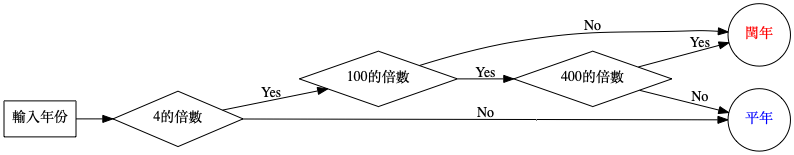
\includegraphics[width=560]{./YearJudge.png}
\caption{\label{fig:YearJudge}
閏年判斷流程}
\end{figure}

\subsubsection{code \#1}
\label{sec:orgc143d99}
\lstset{breaklines=true,language=Python,label= ,caption= ,captionpos=b,numbers=none}
\begin{lstlisting}
year = int(input("請輸入一個年份:"))
if (year % 4) == 0:
    if (year % 100) == 0:
        if (year % 400) == 0:
            print("%s年是世紀閏年" % year)
        else:
            print("%s年為平年" % year)
    else:
        print("%s年是普通閏年" % year)
else:
    print("%s年為平年" % year)
\end{lstlisting}

\subsubsection{code \#2}
\label{sec:orgd8f4671}
\lstset{breaklines=true,language=Python,label= ,caption= ,captionpos=b,numbers=none}
\begin{lstlisting}
year = int(input("請輸入一個年份:"))
if (year % 4) == 0 and (year % 100) !=0 or (year % 400) == 0:
    print("%s年是閏年" % year)
else:
    print("%s年為平年" % year)
\end{lstlisting}

\subsubsection{練習題}
\label{sec:org9412e6f}
\begin{itemize}
\item \href{http://skyoj.tnfsh.tn.edu.tw/sky/index.php/problem/view/162/}{skyoj \#162 成績等第判別}\\
\end{itemize}

\section{迴圈結構}
\label{sec:orgcd4ac4a}

\subsection{for}
\label{sec:orgf603eaa}

\subsubsection{語法}
\label{sec:orgae87cb3}
\lstset{breaklines=true,language=Python,label= ,caption= ,captionpos=b,numbers=none}
\begin{lstlisting}
for variable in List:
    statement 1
    ...
\end{lstlisting}
\begin{itemize}
\item for迴圈的變數會依序走訪序列中的元素\\
\item 序列\footnote{\href{http://liyangbit.com/tutorials/python-list/}{Python數據類型-List介紹} \\}可為range函式、字串(string)、表列(list)、元組(tuple)、字典(dict)、集合(set)\\
\end{itemize}

\subsubsection{List為range() function語法}
\label{sec:org49b9668}
\lstset{breaklines=true,language=Python,label= ,caption= ,captionpos=b,numbers=none}
\begin{lstlisting}
for variable in range([起始值,] 終止值 [,遞增值]):
    statement 1
    ...
\end{lstlisting}
\begin{itemize}
\item 起始值預設為0，遞增值預設為1\\
\item 起始值 ≤ range( )的範圍 < 終止值\\
\end{itemize}

\subsubsection{List為range() function語法}
\label{sec:org88f4708}
\lstset{breaklines=true,language=Python,label= ,caption= ,captionpos=b,firstnumber=1,numbers=left}
\begin{lstlisting}
for x in range(6):
    print(x, end=' ')
print('\n====')
for x in range(3, 10, 2):
    print(x, ' ')
print('\n====')
for x in range(3, 10):
    print(x, end=' ')
\end{lstlisting}

\begin{verbatim}
0 1 2 3 4 5 
====
3  
5  
7  
9  

====
3 4 5 6 7 8 9 
\end{verbatim}

\subsubsection{List為String}
\label{sec:orgcf4af8e}
\lstset{breaklines=true,language=Python,label= ,caption= ,captionpos=b,firstnumber=1,numbers=left}
\begin{lstlisting}
school = 'TNFSH'
for x in school:
    print(x, end=' ')
print('\n=========')
for x in school:
    print(chr(ord(x)+1), end=' ')
\end{lstlisting}

\begin{verbatim}
T N F S H 
=========
U O G T I 
\end{verbatim}


\begin{itemize}
\item ord( ) -> 將字元轉為ASCII編碼(整數)\\
\item chr( ) -> 將ASCII編碼(整數)轉為字元\\
\end{itemize}

\subsection{while}
\label{sec:org946b9b6}
\subsubsection{語法}
\label{sec:orgf52de3c}
\lstset{breaklines=true,language=Python,label= ,caption= ,captionpos=b,numbers=none}
\begin{lstlisting}
while (condition):
    statement 1
    ...
\end{lstlisting}

\subsubsection{範例}
\label{sec:orgf15916a}
\lstset{breaklines=true,language=Python,label= ,caption= ,captionpos=b,firstnumber=1,numbers=left}
\begin{lstlisting}
n = 12345
while (n > 0):
    print(n%10)
    n //= 10
\end{lstlisting}

\begin{verbatim}
5
4
3
2
1
\end{verbatim}


\lstset{breaklines=true,language=Python,label=最大公因數,caption= ,captionpos=b,firstnumber=1,numbers=left}
\begin{lstlisting}
m, n = 42, 75
while (n > 0):
    m, n = n, m % n
print(m)
\end{lstlisting}

\begin{verbatim}
3
\end{verbatim}

\subsection{while + else}
\label{sec:orgdb04cf9}
\subsubsection{語法}
\label{sec:org952ab3a}
\lstset{breaklines=true,language=Python,label= ,caption= ,captionpos=b,numbers=none}
\begin{lstlisting}
while (condition):
    statement 1
    ...
else:
    statement 3
    ...
\end{lstlisting}

\subsubsection{範例}
\label{sec:orgc8549f0}
\lstset{breaklines=true,language=Python,label= ,caption= ,captionpos=b,firstnumber=1,numbers=left}
\begin{lstlisting}
n = 56
while (n%2 == 0):
    print(n, end=' ')
    n //= 2
else:
    print('end with %d' %n)
\end{lstlisting}

\begin{verbatim}
56 28 14 end with 7
\end{verbatim}

\subsection{break}
\label{sec:org3aac5be}
跳出整個loop\\
\subsubsection{範例}
\label{sec:org47ae026}
\lstset{breaklines=true,language=Python,label= ,caption= ,captionpos=b,firstnumber=1,numbers=left}
\begin{lstlisting}
for letter in 'Python':
    if letter == 'h':
        print('Now stop...')
        break
    print('Processing Letrer:', letter)
\end{lstlisting}

\begin{verbatim}
Processing Letrer: P
Processing Letrer: y
Processing Letrer: t
Now stop...
\end{verbatim}

\subsection{continue}
\label{sec:org9e28c9f}
跳出單次loop\\
\subsubsection{範例}
\label{sec:org1e79a14}
\lstset{breaklines=true,language=Python,label= ,caption= ,captionpos=b,firstnumber=1,numbers=left}
\begin{lstlisting}
for letter in 'Python':
    if letter == 'h':
        print('Now skip...')
        continue
    print('Processing Letrer:', letter)
\end{lstlisting}

\begin{verbatim}
Processing Letrer: P
Processing Letrer: y
Processing Letrer: t
Now skip...
Processing Letrer: o
Processing Letrer: n
\end{verbatim}

\subsection{巢狀迴圈}
\label{sec:org9cb029e}
\subsubsection{範例}
\label{sec:org00febcf}
\lstset{breaklines=true,language=Python,label= ,caption= ,captionpos=b,firstnumber=1,numbers=left}
\begin{lstlisting}
for i in range(1, 10):
    for j in range(1, 10):
        print('%d*%d=%2d' %(i, j, i*j), end=' ')
    print()
\end{lstlisting}

\begin{verbatim}
1*1= 1 1*2= 2 1*3= 3 1*4= 4 1*5= 5 1*6= 6 1*7= 7 1*8= 8 1*9= 9 
2*1= 2 2*2= 4 2*3= 6 2*4= 8 2*5=10 2*6=12 2*7=14 2*8=16 2*9=18 
3*1= 3 3*2= 6 3*3= 9 3*4=12 3*5=15 3*6=18 3*7=21 3*8=24 3*9=27 
4*1= 4 4*2= 8 4*3=12 4*4=16 4*5=20 4*6=24 4*7=28 4*8=32 4*9=36 
5*1= 5 5*2=10 5*3=15 5*4=20 5*5=25 5*6=30 5*7=35 5*8=40 5*9=45 
6*1= 6 6*2=12 6*3=18 6*4=24 6*5=30 6*6=36 6*7=42 6*8=48 6*9=54 
7*1= 7 7*2=14 7*3=21 7*4=28 7*5=35 7*6=42 7*7=49 7*8=56 7*9=63 
8*1= 8 8*2=16 8*3=24 8*4=32 8*5=40 8*6=48 8*7=56 8*8=64 8*9=72 
9*1= 9 9*2=18 9*3=27 9*4=36 9*5=45 9*6=54 9*7=63 9*8=72 9*9=81 
\end{verbatim}

\section{資料型別}
\label{sec:org9bd0ac6}
\subsection{字串string}
\label{sec:orgf4fa809}
\subsubsection{資料格式}
\label{sec:orgca6eb70}
以單引號(')或雙引號(")將資料含括起來\\
\subsubsection{範例}
\label{sec:orgae0ecda}
\begin{center}
\begin{tabular}{lrrrrrrrrrr}
\hline
index
左至右 & 0 & 1 & 2 & 3 & 4 & 5 & 6 & 7 & 8 & 9\\
字串 & 0 & 6 & - & 2 & 3 & 7 & 1 & 2 & 0 & 6\\
index
右至左 & -10 & -9 & -8 & -7 & -6 & -5 & -4 & -3 & -2 & -1\\
\hline
\end{tabular}
\end{center}
\subsubsection{字串運算子}
\label{sec:orgc7e1cad}
\begin{itemize}
\item +: 連接字串\\
\item *: 重複字串\\
\item\relax [index]: 字串中index所在字元\\
\item\relax [start:end:increment]: 截取部份字串\\
\item in: 判斷是否為子字串\\
\end{itemize}
\lstset{breaklines=true,language=Python,label= ,caption= ,captionpos=b,firstnumber=1,numbers=left}
\begin{lstlisting}
tel = '06-2371206'
ext = '#600'
# +
print('tel+ext:',tel+ext)
# *
print('ext*2:', ext*2)
# [index]
print('tel[5]:', tel[5])
# [start:end:increment]
print('tel[1:4]:',tel[1:4])
print('tel[6: ]:',tel[6: ])
print('tel[ :6]:',tel[ :6])
print('tel[::-1]:',tel[::-1])
# in
print("'9' in tel:", '9' in tel)
\end{lstlisting}

\begin{verbatim}
tel+ext: 06-2371206#600
ext*2: #600#600
tel[5]: 7
tel[1:4]: 6-2
tel[6: ]: 1206
tel[ :6]: 06-237
tel[::-1]: 6021732-60
'9' in tel: False
\end{verbatim}
\subsubsection{字串function與method}
\label{sec:orgc5b10c4}
\begin{itemize}
\item len(<str>):	計算字串長度\\
\item <str>.lower(): 字串轉小寫\\
\item <str>.upper(): 字串轉大寫\\
\item <str>.islower(): 字串中英文全大寫\\
\item <str>.isupper(): 字串中英文全小寫\\
\item <str>.find(<str1>): 在<str>尋找<str1>，回傳索引值；
若未找到，回傳-1\\
\item <str>.replace(<str1>, <str2>): 將<str>中的<str1>以<str2>取代\\
\item <str>.split([sep]): 字串以sep分割, sep預設值為空白\\
\end{itemize}
\lstset{breaklines=true,language=Python,label= ,caption= ,captionpos=b,firstnumber=1,numbers=left}
\begin{lstlisting}
school = 'Tnfsh'
print('school:', school)
print('len(school):', len(school))
print('school.lower():', school.lower())
print('school.isupper():', school.isupper())
print("school.find('fsh'):", school.find('fsh'))
print("school.replace('fsh', ssh'):", school.replace('fsh', 'ssh'))
school = school.replace('fsh', 'ssh')
print("school.split('f'):", school.split('n'))
\end{lstlisting}

\begin{verbatim}
school: Tnfsh
len(school): 5
school.lower(): tnfsh
school.isupper(): False
school.find('fsh'): 2
school.replace('fsh', ssh'): Tnssh
school.split('f'): ['T', 'ssh']
\end{verbatim}

\subsection{列表list}
\label{sec:org40d707b}
\subsubsection{資料格式}
\label{sec:org903db11}
\begin{itemize}
\item 以[ ]將不同型態的資料含括起來，以 , 分隔\\
\item 表列中的資料是有序排列，從0開始編號\\
\item 格式：表列名稱 = [元素1, 元素2, … ]\\
\end{itemize}
\lstset{breaklines=true,language=Python,label= ,caption= ,captionpos=b,firstnumber=1,numbers=left}
\begin{lstlisting}
data = ['John', [95, 118], 'May', 100]
print(data[1])
\end{lstlisting}

\begin{verbatim}
[95, 118]
\end{verbatim}

\subsubsection{表列函式與方法}
\label{sec:orgcfa43ee}
\begin{itemize}
\item len(<list>): 計算表列元素個數\\
\item list(<str>): 將<str>轉成表列\\
\item <list>.clear():	清除表列中所有元素\\
\item <list>.append(<obj>): 將<obj>加到<list>尾端\\
\item <list>.extend(<list1>): 將<list1>合併至<list>尾端\\
\item <list>.remove(<obj>): 移除<list>中<obj>元素\\
\item <list>.insert(<i>,<obj>): 將<obj>加到<list>的索引值<i>位置\\
\item <list>.pop([index]): 從<list>取出指定元素
若[index]未指定，則取出尾端元素\\
\item <list>.reverse():	反轉表列元素\\
\item sum(<list>): 將表列中所有元素加總(註：僅限表列元素皆為數字)\\
\item <list>.sort(): 將表列中所有元素排序\\
\item '[sep]'.join( <list>): 用[sep]來連結表列元素，若未指定[sep]，則無間隔(僅限表列元素皆為字串)\\
\end{itemize}
\lstset{breaklines=true,language=Python,label= ,caption= ,captionpos=b,firstnumber=1,numbers=left}
\begin{lstlisting}
data = ['John', [95, 118], 'May', 100]
print(len(data))
print(len(data[1]))
print(list('TNFSH'))
data.clear()
print(data)
data.append(35)
print(data)
data1 = [89, 'James', 100]
data.extend(data1)
print(data)
data.remove('James')
print(data)
data.insert(1, 200)
print(data)
data.pop()
data.reverse()
print(data)
print(sum(data))
data.sort()
print(data)
# string
data_s = ["a", "b", "c"]
sep = "-"
print(sep.join(data_s))
\end{lstlisting}

\begin{verbatim}
4
2
['T', 'N', 'F', 'S', 'H']
[]
[35]
[35, 89, 'James', 100]
[35, 89, 100]
[35, 200, 89, 100]
[89, 200, 35]
324
[35, 89, 200]
a-b-c
\end{verbatim}

\subsubsection{練習}
\label{sec:org4c2b827}
\begin{itemize}
\item 連續輸入成績(輸入-1結束)，將成績由高至低排序輸出，並輸出總分、平均\\
\end{itemize}
\lstset{breaklines=true,language=Python,label= ,caption= ,captionpos=b,numbers=none}
\begin{lstlisting}
score = []
while(True):
    sc = int(input())
    if (sc != -1):
        score.append(sc)
    else: 
        break
score.sort(reverse=True)
print(score)
\end{lstlisting}

\begin{itemize}
\item 計算機\\
\end{itemize}
\lstset{breaklines=true,language=Python,label=計算機,caption= ,captionpos=b,firstnumber=1,numbers=left}
\begin{lstlisting}
sum = 0
grades = []
for i in range(0, 5):
    x = int(input("請輸入第" + str(i + 1) + "個成績: "))
    grades.append(x)
    sum += x
print(sum/5)
print(grades)
\end{lstlisting}

\subsection{元組tuple}
\label{sec:orgd957171}
\subsubsection{資料格式}
\label{sec:orga391747}
\begin{itemize}
\item 資料格式：以( )將不同型態的資料含括起來，以 , 分隔\\
\item 元組中的資料是有序排列，從0開始編號\\
\item 格式：元組名稱 = (元素1, 元素2, … )\\
\item 與表列list類似，但元組tuple內的元素不能修改\\
\end{itemize}
\subsubsection{範例}
\label{sec:org6b59e93}
\lstset{breaklines=true,language=Python,label= ,caption= ,captionpos=b,firstnumber=1,numbers=left}
\begin{lstlisting}
data = ( 'John', [95, 118], 'May', 100 )
print(data[1])
tup1 = (53, )    #只有一個元素時，其後要加逗號
print(tup1)
\end{lstlisting}

\begin{verbatim}
[95, 118]
(53,)
\end{verbatim}
\subsubsection{練習: 史上最強掌法}
\label{sec:org6021eb1}
自從鐵掌無敵馬掌門出任武林盟主後，綠林豪傑一片哀鴻，民不聊生，痛苦指數破表，眾家名門弟子甚至遠避異鄉以求溫飽。近來馬掌門更獨創「油電雙掌」，以圖鞏固武林領導地位，此套掌法高深莫測，武林中人聞風喪膽，少林、武當各派高手不得不拋開門戶之見，齊聚「竹園崗」合作商議對策。目前僅由歴來幾次掌下逃生者的對戰經驗分析出以下數據\\
\begin{center}
\begin{tabular}{lr}
與馬掌門對戰時間(秒) & 對戰者每秒接受之傷害值\\
\hline
120以下 & 2.10\\
121\textasciitilde{}330 & 3.02\\
331\textasciitilde{}500 & 4.39\\
501\textasciitilde{}700 & 4.97\\
701以上 & 5.63\\
\end{tabular}
\end{center}
請你幫這些可憐的高手寫一個程式分析對戰時間與受傷指數間的關係。\\
輸入：0 \textasciitilde{} 10000秒之間任意值\\
輸出：受傷指數\\
\subsubsection{解1}
\label{sec:orgc9dec1b}
\lstset{breaklines=true,language=Python,label= ,caption= ,captionpos=b,firstnumber=1,numbers=left}
\begin{lstlisting}
#sec = input()
sec = 800
if sec <= 120:
    print(sec*2.10)
elif sec > 120 and sec <= 330:
    print(120*2.10+(sec-120)*3.02)
elif sec > 330 and sec <= 500:
    print(120*2.10+(330-120)*3.02+(sec-300)*4.39)
elif sec > 500 and sec <= 700:
    print(120*2.10+(330-120)*3.02+(500-330)*4.39+(sec-500)*4.97)
elif sec > 700:
    print(120*2.10+(330-120)*3.02+(500-330)*4.39+(700-500)*4.97+(sec-700)*5.63)
\end{lstlisting}

\begin{verbatim}
3189.5
\end{verbatim}

\subsubsection{解2}
\label{sec:orga59ba5e}
\lstset{breaklines=true,language=Python,label= ,caption= ,captionpos=b,firstnumber=1,numbers=left}
\begin{lstlisting}
#sec = input()
sec = 800
hurt = 0
gap = (700, 500, 330, 120, 0)
rate = (5.63, 4.97, 4.39, 3.02, 2.10)
for i in range(5):
    if sec > gap[i]:
        hurt += (sec-gap[i])*rate[i]
        sec = gap[i]
print(hurt)
\end{lstlisting}

\begin{verbatim}
3189.5
\end{verbatim}

\subsection{字典dict}
\label{sec:orgdaadb98}
\subsubsection{資料格式}
\label{sec:orgaa4aa6e}
\begin{itemize}
\item 以\{ \}將各組鍵:值對應資料含括起來，以 , 分隔\\
\item 字典中的資料是無序的\\
\item 格式：字典名稱 = \{k1:v1, k2:v2,  … \}\\
\item 範例：\\
\item 註：若字典中有相同的key，則會取出最後的value\\
\end{itemize}
\subsubsection{範例}
\label{sec:org73d73dc}
\lstset{breaklines=true,language=Python,label= ,caption= ,captionpos=b,firstnumber=1,numbers=left}
\begin{lstlisting}
data = { 'John': 95,  'May': 100 }
print(data['May'])
\end{lstlisting}

\begin{verbatim}
100
\end{verbatim}
\subsubsection{dic操作}
\label{sec:org7a6f428}
\begin{itemize}
\item 新增、修改、刪除\\
\end{itemize}
\lstset{breaklines=true,language=Python,label= ,caption= ,captionpos=b,firstnumber=1,numbers=left}
\begin{lstlisting}
data = { 'John': 95,  'May': 100 }
# 新增
data['Harrison'] = 88
# 修改
data['John'] = 99
# 刪除鍵值對
del data['John']
print(data)
# 刪除dic
del data
# print(data) --> NameError: name 'data' is not defined
\end{lstlisting}

\begin{verbatim}
{'May': 100, 'Harrison': 88}
\end{verbatim}
\subsubsection{dic method}
\label{sec:orgf9a1776}
\begin{itemize}
\item <dict>.clear()\\
\end{itemize}
\lstset{breaklines=true,language=Python,label= ,caption= ,captionpos=b,firstnumber=1,numbers=left}
\begin{lstlisting}
data = { 'John': 95,  'May': 100, 'John': 105 }
print("data:",data)
print("data.clear():",data.clear())
\end{lstlisting}

\begin{verbatim}
data: {'John': 105, 'May': 100}
data.clear(): None
\end{verbatim}


\begin{itemize}
\item <dict>.copy()\\
\end{itemize}
\lstset{breaklines=true,language=Python,label= ,caption= ,captionpos=b,firstnumber=1,numbers=left}
\begin{lstlisting}
data = { 'John': 95,  'May': 100, 'John': 105 }
data1 = data.copy()
print("data1 = data.copy():",data1.copy())
\end{lstlisting}

\begin{verbatim}
data1 = data.copy(): {'John': 105, 'May': 100}
\end{verbatim}


\begin{itemize}
\item <dict>.get(key, default=None)\\
\item <dict>.items()\\
\item <dict>.keys()\\
\item <dict>.values()\\
\end{itemize}
\lstset{breaklines=true,language=Python,label= ,caption= ,captionpos=b,firstnumber=1,numbers=left}
\begin{lstlisting}
data = { 'John': 95,  'May': 100, 'John': 105 }
print("data.get('John'):",data.get('John'))
print("data.items():",data.items())
print("data.keys():",data.keys())
print("data.values()",data.values())
\end{lstlisting}

\begin{verbatim}
data.get('John'): 105
data.items(): dict_items([('John', 105), ('May', 100)])
data.keys(): dict_keys(['John', 'May'])
data.values() dict_values([105, 100])
\end{verbatim}


\begin{itemize}
\item <dict>.popitem()\\
\end{itemize}
\lstset{breaklines=true,language=Python,label= ,caption= ,captionpos=b,firstnumber=1,numbers=left}
\begin{lstlisting}
data = { 'John': 95,  'May': 100, 'John': 105 }
pop1 = data.popitem()
print(pop1)
\end{lstlisting}

\begin{verbatim}
('May', 100)
\end{verbatim}


\begin{itemize}
\item <dict>.fromkes(<seq>[, val]): Python 字典 fromkeys() 函數用於創建一個新字典，以序列 seq 中元素做字典的鍵，value為字典所有鍵對應的初始值。\\
\end{itemize}
\lstset{breaklines=true,language=Python,label= ,caption= ,captionpos=b,firstnumber=1,numbers=left}
\begin{lstlisting}
data = { 'John': 95,  'May': 100, 'John': 105 }
name = ('Vanissa', 'May', 'John')
data2 = data.fromkeys(name)
print(data2)
data2 = data.fromkeys(name, 100)
print(data2)
\end{lstlisting}

\begin{verbatim}
{'Vanissa': None, 'May': None, 'John': None}
{'Vanissa': 100, 'May': 100, 'John': 100}
\end{verbatim}

\subsection{List v.s. Tuple}
\label{sec:org38384e7}
二者的差異與適用時機\footnote{\href{https://www.programiz.com/python-programming/list-vs-tuples}{Python List vs. Tuples} \\}：\\
\subsubsection{能否改變內容}
\label{sec:org489cfd6}
Using a tuple instead of a list can give the programmer and the interpreter a hint that the data should not be changed.\\
\subsubsection{可讀性}
\label{sec:orgd63eaae}
Reading data is simpler when tuples are stored inside a list. For example,\\
\lstset{breaklines=true,language=Python,label= ,caption= ,captionpos=b,firstnumber=1,numbers=left}
\begin{lstlisting}
[(2,4), (5,7), (3,8), (5,9)]
\end{lstlisting}
is easier to read than\\
\lstset{breaklines=true,language=Python,label= ,caption= ,captionpos=b,firstnumber=1,numbers=left}
\begin{lstlisting}
[[2,4], [5,7], [3,8], [5,9]]
\end{lstlisting}
\subsubsection{與dictionary的相似性}
\label{sec:orgd2d0ec9}
Tuples are commonly used as the equivalent of a dictionary without keys to store data. For Example,\\
\lstset{breaklines=true,language=Python,label= ,caption= ,captionpos=b,firstnumber=1,numbers=left}
\begin{lstlisting}
[('Swordfish', 'Dominic Sena', 2001), ('Snowden', ' Oliver Stone', 2016), ('Taxi Driver', 'Martin Scorsese', 1976)]
\end{lstlisting}
Above example contains tuples inside list which has a list of movies.\\
Tuple can also be used as key in dictionary due to their hashable and immutable nature whereas Lists are not used as key in a dictionary because list can't handle \_\textsubscript{hash}\_\textsubscript{()} and have mutable nature.\\
\lstset{breaklines=true,language=Python,label= ,caption= ,captionpos=b,firstnumber=1,numbers=left}
\begin{lstlisting}
  key_val= {('alpha','bravo'):123} #Valid
key_val = {['alpha','bravo']:123} #Invalid
\end{lstlisting}

\subsection{集合set}
\label{sec:org6f87203}
\subsubsection{資料格式}
\label{sec:orge968fd5}
\begin{itemize}
\item 資料格式：以\{\}將各組資料含括起來，以','分隔,或以set()建立\\
\item 集合中的資料是無序的，會自動刪除重複元素\\
\item 格式：\lstinline[breaklines=true,language=Python]~ 集合名稱 = {元素1, 元素2, … }~\\
\item 註：set(<seq>)函式的參數<seq>可為字串、表列、元組、字典\\
\end{itemize}
\subsubsection{範例}
\label{sec:org69d217b}
\lstset{breaklines=true,language=Python,label= ,caption= ,captionpos=b,firstnumber=1,numbers=left}
\begin{lstlisting}
S1 = { 'John', 95, 'May', 100, 'John' }
		
S2 = set('apple')  ⇒ {'l', 'a', 'e', 'p'}  # 集合的資料是無序的
\end{lstlisting}
\subsubsection{元素新增刪除}
\label{sec:org5104f3b}
\begin{itemize}
\item \lstinline[breaklines=true,language=Python]~<set>.add(<item>)~\\
\item \lstinline[breaklines=true,language=Python]~<set>.remove(<item>)~\\
\item remove()若無此item會發生錯誤\\
\end{itemize}
\lstset{breaklines=true,language=Python,label= ,caption= ,captionpos=b,firstnumber=1,numbers=left}
\begin{lstlisting}
s = set('apple')
s.add('x')
print(s)
s.remove('p')
print(s)
\end{lstlisting}

\begin{verbatim}
{'e', 'p', 'x', 'l', 'a'}
{'e', 'x', 'l', 'a'}
\end{verbatim}
\subsubsection{集合運算}
\label{sec:org71f39bc}
\begin{center}
\begin{tabular}{ll}
運算 & 符號\\
\hline
聯集 & \(\vert{}\)\\
交集 & \&\\
差橆 & -\\
互斥 & \^{}\\
屬於 & in\\
\end{tabular}
\end{center}
\lstset{breaklines=true,language=Python,label= ,caption= ,captionpos=b,firstnumber=1,numbers=left}
\begin{lstlisting}
c = {'1234', 'TNFSH', 'qq', '434'}
print(c)
a = set('1234')
b = set('357')
print("a | b:", a | b)
print("a & b:", a & b)
print("a - b:", a - b)
print("b | a:", b | a)
print("a ^ b:", a ^ b)
print("'5' in a:", '5' in a)
print("'5' in b:", '5' in b)
\end{lstlisting}

\begin{verbatim}
{'1234', 'TNFSH', '434', 'qq'}
a | b: {'4', '2', '1', '5', '7', '3'}
a & b: {'3'}
a - b: {'4', '2', '1'}
b | a: {'4', '5', '2', '1', '7', '3'}
a ^ b: {'4', '2', '7', '5', '1'}
'5' in a: False
'5' in b: True
\end{verbatim}
\subsubsection{詳細語法}
\label{sec:orgf8df7fc}
\begin{itemize}
\item \href{https://www.runoob.com/python3/python3-set.html}{Python3 集合 }\\
\end{itemize}
\subsubsection{練習：\href{http://skyoj.tnfsh.tn.edu.tw/sky/index.php}{skyoj ⇒ Contest ⇒ Python練習題(資料型別)}}
\label{sec:orgde21069}

\subsection{資料型別整理}
\label{sec:org94b376b}
\begin{center}
\begin{tabular}{lllll}
\hline
資料型別 & 符號 & 資料可改? & 資料有序? & 資料類型\\
\hline
字串string & ' ' 或 " " & ✖️ & ✔️ & 相同(字元)\\
表列list & [ ] & ✔️ & ✔️ & 可不同\\
元組tuple & ( ) & ✖ & ️✔ & ️可不同\\
字典dict & \{ \} & ✔️ & ✖️ & 相同(鍵:值)\\
集合set & \{ \} & ✔️ & ✖️ & 可不同\\
\end{tabular}
\end{center}

\section{FUNCTION}
\label{sec:orgb55a24a}
\subsection{函式(function)基本操作}
\label{sec:orgedb29aa}
\subsubsection{函式(function)的重要性}
\label{sec:org4e44574}
\begin{itemize}
\item function為一段程式的集合，可視為一個獨立的區段。\\
\item function可重覆使用，因此為結構化程式語言的重要元素。
可將龐大複雜的程式分解為小問題，由多人分別以function解決，縮短開發時間。\\
\item function可區分為以下三類：\\
\begin{itemize}
\item Python內建function，如: print()、len()、int()、str()\ldots{}。\\
\item 第三方公司所開發的模組module(多個function組合)。\\
\item 自定義function。\\
\end{itemize}
\end{itemize}
\subsubsection{自定義函式}
\label{sec:org476bb24}
\begin{itemize}
\item 宣告語法\\
\end{itemize}
\lstset{breaklines=true,language=Python,label= ,caption= ,captionpos=b,firstnumber=1,numbers=left}
\begin{lstlisting}
def 函式名稱 ( [參數1, 參數2, ...] ):
    程式區塊

    [ return 值 ]
\end{lstlisting}
\begin{itemize}
\item 說明 :\\
\begin{itemize}
\item 參數可省略，亦即呼叫function不需傳入任何資料(引數)。\\
\item 若無回傳值，則無需return。\\
\item 若多個回傳值可用逗號隔開。\\
\end{itemize}
\end{itemize}
\subsubsection{自定義函式的呼叫}
\label{sec:orgcfcc423}
\begin{itemize}
\item 呼叫函式語法：\\
\end{itemize}

\lstset{breaklines=true,language=Python,label= ,caption= ,captionpos=b,firstnumber=1,numbers=left}
\begin{lstlisting}
def circle(r):
    return r*r*3.14;

r = 10
print('半徑%d的圓面積：%d' %(r, circle(r)))
\end{lstlisting}

\begin{verbatim}
半徑10的圓面積：314
\end{verbatim}

\subsubsection{多參數函式}
\label{sec:org9513d55}
\begin{itemize}
\item 呼叫函式時引數(arugment)個數\\
\item 自定義函式的參數(parameter)個數\\
\end{itemize}
設定參數初始值。
若呼叫時無引數傳入，
則使用其初始值。\\
\lstset{breaklines=true,language=Python,label= ,caption= ,captionpos=b,firstnumber=1,numbers=left}
\begin{lstlisting}
def printInfo(name, school='TNFSH'):
    print('學生:',name,'就讀:',school)
    return

printInfo(name='James')
printInfo(name='Harrison',school='TNSSH')
\end{lstlisting}

\begin{verbatim}
學生: James 就讀: TNFSH
學生: Harrison 就讀: TNSSH
\end{verbatim}

\subsubsection{多回傳值函式}
\label{sec:org1f66017}
\begin{itemize}
\item 呼叫函式多個回傳值語法：\\
\begin{itemize}
\item 
\end{itemize}
\end{itemize}
\lstset{breaklines=true,language=Python,label= ,caption= ,captionpos=b,firstnumber=1,numbers=left}
\begin{lstlisting}
def scoreProcessor(score):
    sum = 0
    for x in score:
        sum += x
    return sum, sum/len(score)

scores = (21, 33, 83, 100, 75, 60)
sum, avg = scoreProcessor(scores)
print('sum=',sum,',average=',avg)
\end{lstlisting}

\begin{verbatim}
sum= 372 ,average= 62.0
\end{verbatim}
\subsection{引數(argument)的傳遞}
\label{sec:org6bc8d8c}
\begin{itemize}
\item 每一個函式都是獨立的，所以函式只知道自己程式區域內的變數，不認識函式外的變數。\\
\item 變數因其所宣告位置，可區分為全域變數(Global variable)、區域變數(Local variable)。\\
\begin{itemize}
\item 全域變數：宣告在任何函式外，所有函式皆可存取。\\
\item 區域變數：宣告在函式內，僅函式內可存取。c\\
\end{itemize}
\item 全域變數與區域變數範例\\
\end{itemize}
\lstset{breaklines=true,language=Python,label= ,caption= ,captionpos=b,firstnumber=1,numbers=left}
\begin{lstlisting}
def printGlobal(x, y):
    print(a+b)

def printLocal(a, b):
    print(a+b)

a, b = 5, 10
printGlobal(10, 10)
printLocal(10,10)
\end{lstlisting}

\begin{verbatim}
15
20
\end{verbatim}
\subsubsection{傳值與傳址}
\label{sec:orgf03da6b}
\begin{itemize}
\item 引數(argument)的傳遞分為兩種方式，由Python自動判別：\\
\begin{itemize}
\item 傳值呼叫(Call-by-Value)\\
\item 傳址呼叫(Call-by-Reference)\\
\end{itemize}
\end{itemize}
\begin{center}
\begin{tabular}{llll}
引數傳遞 & 傳遞內容 & 參數改變 & 資料型別\\
\hline
傳值呼叫 call-by-value & 引數值 & 否 & bool, int, float, str, tuple, chr\\
傳址呼叫call-by-reference & 引數記憶體位址 & 是 & list, dict, set\\
\end{tabular}
\end{center}
\lstset{breaklines=true,language=Python,label= ,caption= ,captionpos=b,firstnumber=1,numbers=left}
\begin{lstlisting}
# str傳值、list傳址
def ccc(name, score):
    name = 'Amy'
    score.append(99)
    print('--函式內輸出---')
    print('name:', name,'\tscore:',score)

name = 'Josh'
score = [77, 88]

ccc(name, score)
print('--主程式輸出--')
print('name:', name,'\tscore:',score)
\end{lstlisting}

\begin{verbatim}
--函式內輸出---
name: Amy 	score: [77, 88, 99]
--主程式輸出--
name: Josh 	score: [77, 88, 99]
\end{verbatim}
\subsection{模組(module)}
\label{sec:orgf034179}
\subsubsection{匯入模組語法：}
\label{sec:org53ed063}
\begin{itemize}
\item 

\item 
\end{itemize}
\subsubsection{範例}
\label{sec:org6060744}
\lstset{breaklines=true,language=Python,label= ,caption= ,captionpos=b,firstnumber=1,numbers=left}
\begin{lstlisting}
import random as ran

print(ran.randint(1, 100))
print(ran.randint(1, 100))
print(ran.randint(1, 100))
\end{lstlisting}

\begin{verbatim}
50
78
16
\end{verbatim}

\subsection{遞迴(recursive)}
\label{sec:orgcd0fabc}
\subsubsection{語法}
\label{sec:orgd9c7ec3}
\begin{itemize}
\item 遞迴(recursive)：一個函式直接呼叫函式本身\\
\end{itemize}
\lstset{breaklines=true,language=Python,label= ,caption= ,captionpos=b,firstnumber=1,numbers=left}
\begin{lstlisting}
def fib(n):
    if n == 1 or n == 2:
        return 1
    else:
        return fib(n-1) + fib(n-2)

print('The %d-th Fibonacci number = %d' %(10, fib(10)))
\end{lstlisting}

\begin{verbatim}
The 10-th Fibonacci number = 55
\end{verbatim}

\subsubsection{基本條件}
\label{sec:org7fc4043}
\begin{itemize}
\item 遞迴程式設計要滿足兩條件:\\
\begin{enumerate}
\item 遞迴關係式，如\\
\end{enumerate}
\end{itemize}
\lstset{breaklines=true,language=Python,label= ,caption= ,captionpos=b,firstnumber=1,numbers=left}
\begin{lstlisting}
fib(n) = fib(n-1) + fib(n-2)
sum(n) = n + sum(n-1)

\end{lstlisting}
\begin{enumerate}
\item 遞迴終止式，如\\
\end{enumerate}
\lstset{breaklines=true,language=Python,label= ,caption= ,captionpos=b,firstnumber=1,numbers=left}
\begin{lstlisting}
f(1) = f(2) = 1
sum(0) = 0
\end{lstlisting}
\begin{itemize}
\item 範例:GCD-while\\
\end{itemize}
\lstset{breaklines=true,language=Python,label= ,caption= ,captionpos=b,firstnumber=1,numbers=left}
\begin{lstlisting}
m, n = 20, 50
while (n>0):
    m, n = n, m % n
print(m)
\end{lstlisting}

\begin{verbatim}
10
\end{verbatim}

\subsubsection{範例}
\label{sec:org6b94a2f}
\begin{itemize}
\item 範例:GCD-recursive\\
\end{itemize}
\lstset{breaklines=true,language=Python,label= ,caption= ,captionpos=b,firstnumber=1,numbers=left}
\begin{lstlisting}
def gcd(a, b):
    if b == 0:
        return a
    return gcd(b, a % b)

a, b = 10, 50
print(gcd(a, b))
\end{lstlisting}

\begin{verbatim}
10
\end{verbatim}

\subsubsection{練習}
\label{sec:org7010085}
\begin{itemize}
\item 計算 n! 值。
輸入 n，輸出 n! = XXXXX。如輸入5，輸出5! = 120。\\
\item 計算C(n, r)組合數。
輸入 n, r，輸出C(n, r) = XX。如輸入9, 4，輸出C(9, 4) = 126。\\
\item 計算擴展歐幾里德。
輸入 a, b，輸出a*x + b*y = gcd。如輸入3, 5，輸出3*2 + 5*-1 = 1\\
\end{itemize}
\lstset{breaklines=true,language=Python,label= ,caption= ,captionpos=b,firstnumber=1,numbers=left}
\begin{lstlisting}
def ext_euclid(a, b):
    old_s,s=1,0
    old_t,t=0,1
    old_r,r=a,b
    if b == 0:
        return 1, 0, a
    else:
        while(r!=0):
            q=old_r//r
            old_r,r=r,old_r-q*r
            old_s,s=s,old_s-q*s
            old_t,t=t,old_t-q*t
    return old_s, old_t, old_r

a, b, c = ext_euclid(240, 33)
print('%dx + %dy = %d' %(a, b, c))
\end{lstlisting}

\begin{verbatim}
4x + -29y = 3
\end{verbatim}

\section{Numpy模組}
\label{sec:orgb9d16fc}
\subsection{匯入模組}
\label{sec:org3535644}
\begin{itemize}
\item 使用模組裡的函式要加模組名稱，如 numpy.arrry( )。例：\lstinline[breaklines=true,language=Python]~ import numpy
~\\
\item 匯入numpy模組並使用np作為簡寫，這是Numpy官方倡導的寫法\lstinline[breaklines=true,language=Python]~ import numpy as np
~\\
\item Numpy中的多維資料型別稱為ndarray\\
\end{itemize}
\subsection{Create ndarray}
\label{sec:orge84222e}
\subsubsection{一維陣列}
\label{sec:org16d5d69}
\begin{itemize}
\item list 或 tuple 轉入\\
\end{itemize}
\lstset{breaklines=true,language=Python,label= ,caption= ,captionpos=b,firstnumber=1,numbers=left}
\begin{lstlisting}
import numpy as np
np1 = np.array( [1, 2, 3, 4] )
print(np1)
\end{lstlisting}

\begin{verbatim}
[1 2 3 4]
\end{verbatim}


\begin{itemize}
\item 使用 np.arange( ) 方法\\
\end{itemize}
\lstset{breaklines=true,language=Python,label= ,caption= ,captionpos=b,firstnumber=1,numbers=left}
\begin{lstlisting}
import numpy as np
np2 = np.arange(5)
print(np2)
\end{lstlisting}

\begin{verbatim}
[0 1 2 3 4]
\end{verbatim}
\subsubsection{多維陣列}
\label{sec:orgbdc7c11}
\begin{itemize}
\item 二維陣列\\
\end{itemize}
\lstset{breaklines=true,language=Python,label= ,caption= ,captionpos=b,firstnumber=1,numbers=left}
\begin{lstlisting}
import numpy as np
np4 = np.array( [[1, 2, 4], [3,4,5]])
print('np4:', np4)

np5 = np.array([np.arange(3), np.arange(3)])
print('np5:', np5)

np6 = np.arange(8).reshape(2, 4)
print('np6:', np6)
\end{lstlisting}

\begin{verbatim}
np4: [[1 2 4]
 [3 4 5]]
np5: [[0 1 2]
 [0 1 2]]
np6: [[0 1 2 3]
 [4 5 6 7]]
\end{verbatim}

\begin{itemize}
\item 多維陣列\\
\end{itemize}
\lstset{breaklines=true,language=Python,label= ,caption= ,captionpos=b,firstnumber=1,numbers=left}
\begin{lstlisting}
import numpy as np

np7 = np.arange(24).reshape(2, 3, 4)
print('np7:',np7)
\end{lstlisting}

\begin{verbatim}
np7: [[[ 0  1  2  3]
  [ 4  5  6  7]
  [ 8  9 10 11]]

 [[12 13 14 15]
  [16 17 18 19]
  [20 21 22 23]]]
\end{verbatim}

\begin{itemize}
\item 隨機矩陣\\
\end{itemize}
\lstset{breaklines=true,language=Python,label= ,caption= ,captionpos=b,firstnumber=1,numbers=left}
\begin{lstlisting}
import numpy as np

np8 = np.random.random( (3, 2)) #矩陣大小以tuple表示
print('np8:', np8)

np9 = np.random.randint( 0, 100, size=[4, 3]) #矩陣大小以list表示
print('np9:', np9)
\end{lstlisting}

\begin{verbatim}
np8: [[0.04349769 0.48755705]
 [0.50627204 0.56730179]
 [0.56445113 0.31159334]]
np9: [[53 73 52]
 [60 58 33]
 [69 89 98]
 [17 92 90]]
\end{verbatim}
\subsection{矩陣運算}
\label{sec:org09b382c}
\lstset{breaklines=true,language=Python,label= ,caption= ,captionpos=b,firstnumber=1,numbers=left}
\begin{lstlisting}
import numpy as np

A = np.array([
    [5, 3, 7],
    [0, 1, -6]
])

B = np.array([
    [1, 2, 3],
    [-1, -2, -3]
])

C = np.array([
    [1, 2],
    [-1, -2],
    [0, 5]
])

k = -3

print('---A+B---\n', A+B)
print('---A-B---\n', A-B)
print('---k*B---\n', k*B)
print('---A.dot(C)---\n', A.dot(C))
\end{lstlisting}

\begin{verbatim}
---A+B---
 [[ 6  5 10]
 [-1 -1 -9]]
---A-B---
 [[ 4  1  4]
 [ 1  3 -3]]
---k*B---
 [[-3 -6 -9]
 [ 3  6  9]]
---A.dot(C)---
 [[  2  39]
 [ -1 -32]]
\end{verbatim}

\subsection{特殊矩陣}
\label{sec:orgfc9b491}
\begin{itemize}
\item 元素全為0矩陣：\lstinline[breaklines=true,language=Python]~ np.zeros(<大小>, <資料型別>) ~\\
\item 元素全為1矩陣：\lstinline[breaklines=true,language=Python]~ np.ones(<大小>, <資料型別>)
# 矩陣大小以 tuple 指定 ~\\
\item 單位矩陣(Identity)：\lstinline[breaklines=true,language=Python]~ np.eye(<m>, <資料型別>)   # eye 與 I 同音 ~\\
\item 反矩陣(Inverse)：\lstinline[breaklines=true,language=Python]~ np.linalg.inv(<矩陣>) 
# 行列式不可為0 ~\\
\end{itemize}
\lstset{breaklines=true,language=Python,label= ,caption= ,captionpos=b,firstnumber=1,numbers=left}
\begin{lstlisting}
import numpy as np

print('np.zeros:\n', np.zeros((3,5), dtype='int'))
print('np.ones:\n', np.ones((3,5), dtype='int'))
print('np.eyes:\n', np.eye(4, dtype='int'))
x = np.random.randint( 0, 10, size=[3, 3])
print('x:\n', x)
xt = x.T # 轉置
print('xt:\n', xt)
mat = xt.dot(x)
print('mat:\n', mat)
print('np.linalg.inv(mat):\n', np.linalg.inv(mat))

\end{lstlisting}

\begin{verbatim}
np.zeros:
 [[0 0 0 0 0]
 [0 0 0 0 0]
 [0 0 0 0 0]]
np.ones:
 [[1 1 1 1 1]
 [1 1 1 1 1]
 [1 1 1 1 1]]
np.eyes:
 [[1 0 0 0]
 [0 1 0 0]
 [0 0 1 0]
 [0 0 0 1]]
x:
 [[5 7 1]
 [2 8 6]
 [1 6 3]]
xt:
 [[5 2 1]
 [7 8 6]
 [1 6 3]]
mat:
 [[ 30  57  20]
 [ 57 149  73]
 [ 20  73  46]]
np.linalg.inv(mat):
 [[ 0.48628827 -0.37053571  0.37659439]
 [-0.37053571  0.3125     -0.33482143]
 [ 0.37659439 -0.33482143  0.38934949]]
\end{verbatim}
\subsection{ndarray屬性}
\label{sec:org8803a3d}
\begin{itemize}
\item dtype：ndarray每個元素的資料型別 (可於創建矩陣時同時指定)\\
\begin{itemize}
\item int, float, bool, D(複數)\\
\end{itemize}
\item ndim：ndarray的維度\\
\item shape：ndarray的大小，即矩陣 m*n ( m 列 n 行 )\\
\item size：ndarray的元素個數\\
\item itemsize：ndarray中每個元素記憶體大小(單位byte)\\
\end{itemize}
\lstset{breaklines=true,language=Python,label= ,caption= ,captionpos=b,firstnumber=1,numbers=left}
\begin{lstlisting}
import numpy as np

np1 = np.arange(12, dtype='D').reshape(3, 2, 2)
print(np1)
print('dtype=', np1.dtype)
print('shape=', np1.shape)
print('size=', np1.size)
print('itemsize=', np1.itemsize)
print('nbytes=', np1.nbytes)
\end{lstlisting}

\begin{verbatim}
[[[ 0.+0.j  1.+0.j]
  [ 2.+0.j  3.+0.j]]

 [[ 4.+0.j  5.+0.j]
  [ 6.+0.j  7.+0.j]]

 [[ 8.+0.j  9.+0.j]
  [10.+0.j 11.+0.j]]]
dtype= complex128
shape= (3, 2, 2)
size= 12
itemsize= 16
nbytes= 16.0
\end{verbatim}

\begin{itemize}
\item nbytes：ndarray的記憶體大小(單位byte)\\
\begin{itemize}
\item real 和 imag：複數的實部和虛部\\
\item real 回傳複數的實部\\
\end{itemize}
\item imag 回傳複數的虛部\\
\item T：矩陣轉置\\
\end{itemize}
\subsubsection{練習}
\label{sec:org61cf188}
\begin{itemize}
\item 使用 random 函式產生 3*5 的矩陣 A\\
\item 使用 randint 函式產生 5*3 的矩陣 B\\
\item 使用 arange 和 reshape 函式產生 3*5 的矩陣 C\\
\item 使用 list 自建 5*3 的矩陣 D\\
\item 計算 10*A + C 和 B - D\\
\item 計算 B•C 和 C•D\\
\item 比較 (B•C)T 和 CT•BT 是否相同?\\
\item 求矩陣 E 的反矩陣\\
\end{itemize}
\subsection{矩陣形狀轉換}
\label{sec:org12eef66}
\begin{itemize}
\item reshape(m, n, …)：不改變原矩陣形狀\\
\item resize(m, n, …)：和 reshape 類似，但會改變原矩陣形狀\\
\item ravel( ) / flatten( )：將多維矩陣轉換成一維矩陣，原矩陣不變\\
\item shape = (m, n, …)：用 tuple 來指定矩陣大小，會改變原矩陣\\
\end{itemize}

\section{Matplotlib}
\label{sec:org9e1a8af}

\section{網路爬蟲}
\label{sec:org66e6fe9}
\lstset{breaklines=true,language=Python,label= ,caption= ,captionpos=b,firstnumber=1,numbers=left}
\begin{lstlisting}

import urllib.request as req
url = "https://huodalife.pixnet.net/blog/"
# 幫request加上一個header
request = req.Request(url, headers = {
    "User-Agent":"Mozilla/5.0 (Macintosh; Intel Mac OS X 10.14; rv:72.0) Gecko/20100101 Firefox/72.0"
})

with req.urlopen(request) as response:
    data = response.read().decode("utf-8")

import bs4
root = bs4.BeautifulSoup(data,"html.parser")

titles = root.find_all("li", class_="title")
pubs = root.find_all("li", class_="publish")
for pub, title in zip(pubs, titles):
    print(pub.span.string,title.a.string)
\end{lstlisting}

\section{Python學習資源}
\label{sec:org51da2da}
\begin{itemize}
\item \href{https://www.runoob.com/python3/python3-tutorial.html}{Python 3教程}\\
\item \href{http://liyangbit.com/tutorials/}{Python教程}\\
\end{itemize}


\section{0802 CNN}
\label{sec:orgd891d86}
\url{https://reurl.cc/Y2gKo}: 各種常用的library, function\\

\section{以python下載網路資料}
\label{sec:org511e72b}
\begin{itemize}
\item import urllib.request as req\\
\end{itemize}

\section{網路爬蟲}
\label{sec:org244a27d}
\subsection{parse HTML}
\label{sec:org2758d29}
\begin{itemize}
\item what is HTML\\
\item 精神：將程式模仿成一般user\\
\end{itemize}
\subsubsection{所需套件}
\label{sec:org8c97dc7}
\begin{itemize}
\item BeautifulSoup\\
\end{itemize}
pip install beautifulsoup4\\
\subsection{範例: 以程式抓取PTT電影板header}
\label{sec:org5997aa3}
\subsubsection{原則}
\label{sec:orgfa24990}
\begin{enumerate}
\item 要抓網路資料，就要先仔細觀察網頁內容\\
\item 要儘量欺騙網站自己是browser\\
\end{enumerate}
\subsubsection{實作: 取得HTML資料}
\label{sec:orgda8a041}
\begin{enumerate}
\item 第一版
\label{sec:org605a279}
\lstset{breaklines=true,language=Python,label= ,caption= ,captionpos=b,firstnumber=1,numbers=left}
\begin{lstlisting}
# 抓取PTT電影版header
import urllib.request as req
url = "https://www.ptt.cc/bbs/Stock/index.html"

with req.urlopen(url) as response:
    data = response.read().decode("utf-8")
print(data)
\end{lstlisting}

\begin{verbatim}
urllib.error.HTTPError: HTTP Error 403: Forbidden
\end{verbatim}

被拒絕原因：這隻程式的行為不像一般使用者，被網站伺服器拒絕。403 Forbidden 是HTTP協議中的一個HTTP狀態碼（Status Code）。可以簡單的理解為沒有權限訪問此站，服務器收到請求但拒絕提供服務\footnote{\href{https://zh.wikipedia.org/wiki/HTTP\_403}{維基百科: HTTP 403} \\}。\\

\item 第二版:加入header
\label{sec:org9c61dae}
\lstset{breaklines=true,language=Python,label= ,caption= ,captionpos=b,firstnumber=1,numbers=left}
\begin{lstlisting}
import urllib.request as req
url = "https://www.ptt.cc/bbs/Stock/index.html"
# 幫request加上一個header
request = req.Request(url, headers = {
    "User-Agent":"Mozilla/5.0 (Macintosh; Intel Mac OS X 10.14; rv:72.0) Gecko/20100101 Firefox/72.0"
})

with req.urlopen(request) as response:
    data = response.read().decode("utf-8")
print('所取得的資料型態：',type(data))
print(data[700:1000])
\end{lstlisting}

\begin{verbatim}
所取得的資料型態： <class 'str'>
er">
	<div id="topbar" class="bbs-content">
		<a id="logo" href="/bbs/">批踢踢實業坊</a>
		<span>&rsaquo;</span>
		<a class="board" href="/bbs/Stock/index.html"><span class="board-label">看板 </span>Stock</a>
		<a class="right small" href="/about.html">關於我們</a>
		<a class="right small" href="/contact.html">
\end{verbatim}
\end{enumerate}

\subsubsection{實作：解析HTML資料內容}
\label{sec:orgc9ac3bb}
\begin{enumerate}
\item 安裝解析HTML所需套件
\label{sec:orge8924b5}
\lstset{breaklines=true,language=shell,label= ,caption= ,captionpos=b,numbers=none}
\begin{lstlisting}
pip install beautifulsoup4
\end{lstlisting}

\item 第三版: 解析HTML
\label{sec:org03a9c29}
\lstset{breaklines=true,language=Python,label= ,caption= ,captionpos=b,firstnumber=1,numbers=left}
\begin{lstlisting}
import urllib.request as req
url = "https://www.ptt.cc/bbs/Stock/index.html"
# 幫request加上一個header
request = req.Request(url, headers = {
    "User-Agent":"Mozilla/5.0 (Macintosh; Intel Mac OS X 10.14; rv:72.0) Gecko/20100101 Firefox/72.0"
})

with req.urlopen(request) as response:
    data = response.read().decode("utf-8")

import bs4
root = bs4.BeautifulSoup(data,"html.parser")
print(root.title)
titles = root.find("div", class_="title")
print(titles)
print(titles.a.string)
titles = root.find_all("div", class_="title")
print(titles)
for title in titles:
    if title.a != None:
        print(title.a.string)
\end{lstlisting}

\begin{verbatim}
<title>看板 Stock 文章列表 - 批踢踢實業坊</title>
<div class="title">
<a href="/bbs/Stock/M.1581985895.A.742.html">Re: [新聞] 蝗蟲抵達邊境 中國人自信：威脅不大</a>
</div>
Re: [新聞] 蝗蟲抵達邊境 中國人自信：威脅不大
[<div class="title">
<a href="/bbs/Stock/M.1581985895.A.742.html">Re: [新聞] 蝗蟲抵達邊境 中國人自信：威脅不大</a>
</div>, <div class="title">
<a href="/bbs/Stock/M.1581986080.A.0B9.html">[新聞] 武漢肺炎衝擊 蘋果率先示警營收無法達標</a>
</div>, <div class="title">
<a href="/bbs/Stock/M.1581987000.A.EE7.html">[新聞] 超預期 國巨MLCC漲價五成</a>
</div>, <div class="title">
<a href="/bbs/Stock/M.1581987018.A.192.html">[新聞] 武漢肺炎》上海美國商會：1/3企業若工廠</a>
</div>, <div class="title">
<a href="/bbs/Stock/M.1581987846.A.95F.html">[新聞] 中芯國際14nm第二代FinFET批量須等到2020</a>
</div>, <div class="title">
<a href="/bbs/Stock/M.1581989947.A.392.html">Re: [請益] 有人買股票而完全捨棄定存嗎?</a>
</div>, <div class="title">
<a href="/bbs/Stock/M.1581990753.A.EB3.html">[新聞] 斷絕華為貨源！美擬祭禁令限制中企取得</a>
</div>, <div class="title">
<a href="/bbs/Stock/M.1581994926.A.A50.html">[標的] 6531愛普</a>
</div>, <div class="title">
<a href="/bbs/Stock/M.1581996309.A.C55.html">[請益] 是不是該立法更限制外資匯出資金？</a>
</div>, <div class="title">
<a href="/bbs/Stock/M.1581999672.A.14E.html">Re: [請益] 存股標的選擇</a>
</div>, <div class="title">
<a href="/bbs/Stock/M.1582000361.A.6A2.html">[標的] 1201 味全 多</a>
</div>, <div class="title">
<a href="/bbs/Stock/M.1582000701.A.2AB.html">Re: [新聞] 蝗蟲抵達邊境 中國人自信：威脅不大</a>
</div>, <div class="title">
<a href="/bbs/Stock/M.1582001420.A.3B8.html">[新聞] 用電大戶買綠電 電證分離更活絡</a>
</div>, <div class="title">
<a href="/bbs/Stock/M.1422199105.A.84E.html">[公告] 精華區導覽Q&amp;A</a>
</div>, <div class="title">
<a href="/bbs/Stock/M.1541252211.A.8BE.html">[公告] Stock 板規V2.6             (2019/06/20)</a>
</div>, <div class="title">
<a href="/bbs/Stock/M.1579935755.A.395.html">[公告] 關於武漢肺炎新聞規範</a>
</div>, <div class="title">
<a href="/bbs/Stock/M.1581919202.A.CF2.html">[閒聊] 2020/02/17 盤後閒聊</a>
</div>, <div class="title">
<a href="/bbs/Stock/M.1581985803.A.F3E.html">[閒聊] 2020/02/18 盤中閒聊</a>
</div>]
Re: [新聞] 蝗蟲抵達邊境 中國人自信：威脅不大
[新聞] 武漢肺炎衝擊 蘋果率先示警營收無法達標
[新聞] 超預期 國巨MLCC漲價五成
[新聞] 武漢肺炎》上海美國商會：1/3企業若工廠
[新聞] 中芯國際14nm第二代FinFET批量須等到2020
Re: [請益] 有人買股票而完全捨棄定存嗎?
[新聞] 斷絕華為貨源！美擬祭禁令限制中企取得
[標的] 6531愛普
[請益] 是不是該立法更限制外資匯出資金？
Re: [請益] 存股標的選擇
[標的] 1201 味全 多
Re: [新聞] 蝗蟲抵達邊境 中國人自信：威脅不大
[新聞] 用電大戶買綠電 電證分離更活絡
[公告] 精華區導覽Q&A
[公告] Stock 板規V2.6             (2019/06/20)
[公告] 關於武漢肺炎新聞規範
[閒聊] 2020/02/17 盤後閒聊
[閒聊] 2020/02/18 盤中閒聊
\end{verbatim}
\end{enumerate}

\subsection{參考資料}
\label{sec:orge8a81b9}
\begin{itemize}
\item \url{https://www.youtube.com/watch?v=9Z9xKWfNo7k}\\
\end{itemize}


\section{如何把python程式publish成網站應用程式}
\label{sec:org0b5a711}
\end{document}
